\documentclass{beamer}
\usetheme{Madrid}

\usepackage{amsmath,amssymb,amsfonts,amsthm}
\usepackage{graphicx}
\usepackage{listings}
\usepackage{gensymb}
\usepackage[utf8]{inputenc}
\usepackage{hyperref}
\usepackage{gvv}

\begin{document}

\title{7-7.2-25}
\author{EE24BTECH11027 - G.V.Satwika}
\date{}
\frame{\titlepage}

\begin{frame}
\frametitle{Problem statement}
Find the equation of a circle passing through the point \brak{7,3} having radius 3 units and whose centre lies on the line $y=x-1$.\\
\end{frame}

\begin{frame}[allowframebreaks]
\frametitle{Solution}
\begin{table}[htbp]
	\centering
	\def\arraystretch{1.5}
	\begin{tabular}[12pt]{ |c| c|}
    \hline
    \textbf{Variable} & \textbf{Description}\\ 
    \hline
    $P$ & point vector\\
    \hline 
    $-u$ & centre of the circle\\
    \hline
    $r$ & radius of the circle\\
    \hline 
    \end{tabular}

	\caption{Variables}
	\label{tab:variables}
\end{table}
From the given information, the following equations can be formulated using the circle equation 
\begin{align}
	\norm{x}^2 + 2u^\top x + f &= 0\\
	\norm{P}^2 + 2u^\top P + f &= 0\label{eq:0.2}\\ 
	\norm{u}^2 - f &= r^2\label{eq:0.3}
\end{align}
From \eqref{eq:0.2} and \eqref{eq:0.3}
\begin{align}
	\norm{P}^2 + 2u^\top P + \norm{u}^2 &= r^2 	
\end{align}
Substituting the values of $u$,$P$ and $r$,
\begin{align}
	2k^2-2k+1+6-20k+7^2+3^2-3^2 &=0 \\
	2k^2-22k+56 &=0 \\
	k &=7,4
\end{align}
resulting in circles with centres 
\begin{align}
	-u&=\myvec{7\\6} or \myvec{4\\3}	
\end{align}
\end{frame}
\begin{frame}
\frametitle{Plot}
\begin{figure}[htbp]
	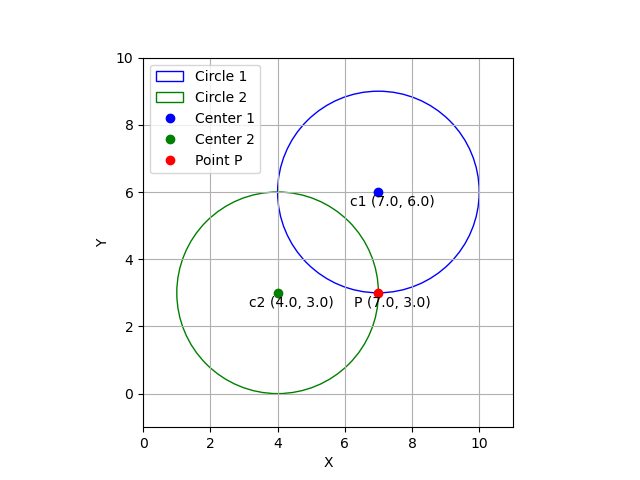
\includegraphics[width=0.75\columnwidth]{figs/circle_plot.png}
	\caption{Plot of circles}
	\label{fig:bode}
\end{figure}
\end{frame}
% Define colors for syntax highlighting
\definecolor{codegreen}{rgb}{0,0.6,0}
\definecolor{codegray}{rgb}{0.5,0.5,0.5}
\definecolor{codepurple}{rgb}{0.58,0,0.82}
\definecolor{backcolour}{rgb}{0.95,0.95,0.92}
% Settings for the C code
\lstset{
    language=C,
    basicstyle=\footnotesize\ttfamily,
    backgroundcolor=\color{backcolour},
    commentstyle=\color{codegreen},
    keywordstyle=\color{blue},
    numberstyle=\tiny\color{codegray},
    stringstyle=\color{codepurple},
    breakatwhitespace=false,
    breaklines=true,
    captionpos=b,
    keepspaces=true,
    numbers=left,
    numbersep=5pt,
    showspaces=false,
    showstringspaces=false,
    showtabs=false,
    tabsize=2
}
\begin{frame}[fragile,allowframebreaks]
\frametitle{C Code}
\lstinputlisting[label=mycode1]{codes/circle.c}
\end{frame}
% Define colors for syntax highlighting
\definecolor{codegreen}{rgb}{0,0.6,0}
\definecolor{codegray}{rgb}{0.5,0.5,0.5}
\definecolor{codepurple}{rgb}{0.58,0,0.82}
\definecolor{backcolour}{rgb}{0.95,0.95,0.92}

% Python style for highlighting
\lstset{
    language=Python,
    basicstyle=\ttfamily\small,
    keywordstyle=\color{blue},
    stringstyle=\color{codepurple},
    commentstyle=\color{codegreen},
    backgroundcolor=\color{backcolour},
    breaklines=true,
    breakatwhitespace=true,
    tabsize=4
}

\begin{frame}[fragile,allowframebreaks]
\frametitle{Python Code}
\lstinputlisting[label=mycode1]{codes/plot.py}
\end{frame}
\end{document}
